章节3和章节4详细介绍了本文提出的方法及其系统设计与实现,最后实现了一个能够从Stack Overflow帖子中识别出API描述性知识句子,并从中迭代抽取API描述性知识的系统。为了对本文提出的方法进行多方面的评估,本章节将会介绍本文设计的一系列实验,以及实验的结果。本章节设计的实验主要是为了回答以下3个问题:
\begin{enumerate}
    \item RQ1:API描述性知识抽取系统中的各个模块工作效果如何,其输出质量如何?
    \item RQ2:从不同的方面对本方法抽取出来的API描述性知识进行评估,其有效性如何?
    \item RQ3:本方法抽取出来的API描述性知识能否对API文档进行补充。
\end{enumerate}

\section{语料库生成模块质量评估}
本章节将对API描述性知识抽取系统中的语料库生成模块进行实验评估。

\subsection{实验设计}
本节所设计的实验用于评估用于语料库的质量,评估重点在训练的fastText二分类器能否正确的识别出Stack Overflow中的API描述性知识句子。本文从完成分句后经过过滤的带有API提及的句子列表中随机采样2000个句子,并邀请了两位具有3年以上Java开发经验的硕士研究生,对这些句子进行独立标注,判断这些句子是否是API描述性知识句子。对于两位标注者的标注结果中不同的部分,邀请第三位标注者对这些不同的部分进行仲裁,并将仲裁结果作为最终的标注结果。

句子标注的结果如表\ref{fig:fig1}所示。在完成句子标注后,本文还需要对两位标注者的共识率进行检验。本文计算出两位标注者的Cohen's kappa指数,用于表示两位标注者的共识率。其计算方法如公式5.1所示:

\begin{equation}
    k=\frac{p_{o}-p_{e}}{1-p_{e}}
\end{equation}

其中,$p_{o}$为实际共识率,$p_{e}$为理论共识率。根据标注数据计算得出的Cohen's kappa系数为0.86,因此我们可以认为两位标注者对于API描述性知识句子标注的共识基本是一致的。

\begin{table}[h]
    \centering
    \caption{API描述性知识句子标注结果}
    \label{fig:fig1}
    \begin{tabular}{|l|l|l|l|}
    \hline
          & 标注者1 & 标注者2 & 仲裁结果 \\ \hline
    正样本数量 & 533  & 580  & 542  \\ \hline
    负样本数量 & 1467 & 1420 & 1458 \\ \hline
    \end{tabular}
    \end{table}

如前文章节4.1.3所述,在得到标注数据后本文还会使用nlpaug工具进行数据扩充,以保证标注数据训练出来的文本分类器的有效性。

在完成扩充后,本方法得到了正样本1626条,负样本1458条,共3084条数据。接着,使用十折交叉验证法来验证使用这些数据训练得到的文本分类器是否有效。十折交叉验证法将会把所有标注数据分为10份,分别取其中一份作为测试集,剩余九份作为训练集,训练10次从而得到十个模型,然后使用各自的测试集来测试十次训练得到的模型的准确度。十折交叉验证得到的召回率、准确率和F值如表\ref{fig:fig2}所示。

\begin{center}
    \begin{table}[h]
        \centering
        \caption{十折交叉验证数据结果}
        \label{fig:fig2}
        \begin{tabular}{cccccccccccc}
        \hline
        模型  & 1    & 2    & 3    & 4    & 5    & 6    & 7    & 8    & 9    & 10   & 平均值  \\ \hline
        准确率 & 0.74 & 0.75 & 0.75 & 0.77 & 0.73 & 0.74 & 0.75 & 0.75 & 0.76 & 0.74 & 0.75 \\
        召回率 & 0.79 & 0.80 & 0.80 & 0.87 & 0.81 & 0.81 & 0.81 & 0.80 & 0.80 & 0.79 & 0.81 \\
        F值  & 0.77 & 0.78 & 0.78 & 0.81 & 0.77 & 0.77 & 0.78 & 0.78 & 0.78 & 0.76 & 0.78 \\ \hline
        \end{tabular}
        \end{table}
\end{center}


\subsection{实验结果分析}
从十折交叉验证的结果来看,fastText二分类器的分类效果较好,平均分类准确率达到75\%,平均召回率达到了81\%。在本方法中,对于分类器分类错误的情况,本文更希望是一个负样本被识别为正样本,而不是相反的情况。这是因为文本分类器对语料库只是进行一个挖掘前的初筛,如果一个非API描述性知识句子被加入语料库中,它有可能在挖掘过程中完全没有被匹配上,这样对本方法的抽取结果就不会造成影响。而如果一个API描述性知识句子被分类成负样本,那么本方法就完全没有机会抽取到这个句子中包含的API描述性知识,同时还无法抽取得到它的语言模式及其变异,这对于本方法是一种损失。从以上实验数据中可以得知,该分类模型的召回率比准确率更高,而召回率通常用于衡量一个分类器对正样本的识别能力,准确率通常用于衡量分类器对负样本的区分能力。因此,可以认为该模型在本方法中对正样本的识别能力是较为出色的。

对fastText二分类器分类错误的数据进行分析,主要原因有:
\begin{enumerate}
    \item 句子中出现了API描述性知识句子中的高频词。如“I override the getPreferredSize() to return the appropriate dimension.”,这个句子包含了常在API描述性知识句子中出现的词汇“override”和“return”,但这个句子的语义更倾向于描述作者的行为,而非API的表现知识,故它虽然不是一个API描述性句子但被分类成了正样本。
    \item 分句错误导致的低质量句子分类错误。如“A ReentrantLock is owned by the thread last successfully locking, but not yet unlocking it.A thread invoking lock will return, successfully acquiring the lock, when the lock is not owned by another thread. The method will return immediately if the current thread already owns the lock.”,由于原帖子的作者在编写时对标点符号的使用较为随意(没有在句号后面加上空格),导致本文修改后的spaCy解析工具将整段话作为一个完整的句子,句子的长度过长,且没有出现非常明显的特征词汇,所以虽然其中存在API描述性句子,但仍然被分类成负样本。
\end{enumerate}

\subsection{语料库质量评估实验总结}
通过以上实验评估,可以认为本系统中的语料库生成模块的性能较好,能够作为API描述性知识抽取的基础。高质量的语料库一定程度上提高了抽取主体模块的输出质量。当语料库中的一个句子能够和抽取主体模块输入的种子API描述性知识元组匹配上,或者与其他API描述性知识句子的语言模式相似时,它是一个有效的API描述性知识的可能性非常高。限制提高语料库质量的瓶颈主要在训练数据的质量和自然语言处理工具上,如果之后能将文章语法不够严谨的帖子筛选掉,或者定制更智能的自然语言分句规则,那么fastText二分类器的分类效果或许能有所提升。

\section{抽取主体模块质量评估}
本章节将对系统中的抽取主体模块进行质量评估。

\subsection{实验设计}
为了验证抽取主体模块的有效性,本实验从句子语料库中随机采样了50个句子,其中35个是API描述性知识句子,另外15个句子不是API描述性知识句子,但在句子中包含有API提及。然后人工总结出这35个句子的API描述性知识元组,从其中随机选择5个作为种子API描述性知识元组,再将这些句子和种子知识元组作为抽取主体模块的输入,进行迭代抽取。抽取过程中,每一轮的抽取结果都会被保存下来,直到程序无法从语料库中抽取出新的知识元组和知识实例为止。通过观察对比每一轮抽取的结果与人工总结的API描述性知识元组,可以对本模块的输出质量进行评估。

\subsection{实验结果分析}
本实验每一轮迭代运行中抽取出来的API描述性知识数量如表\ref{fig:fig3}所示。在第4轮抽取的时候,没有新的API描述性知识元组被抽取出来,抽取流程终止。从抽取出来的知识元组数量分析,从5个种子API描述性知识出发经过3轮迭代可以抽取得到16个的新的知识元组。在结果中,还存在着从非API描述性知识句子中抽取出了错误的API描述性知识元组,这种错误的知识元组有2个。去掉错误的API描述性知识元组,可以计算得出本模块对测试数据的抽取覆盖率为14/30=0.47。

\begin{table}[h]
    \centering
    \caption{抽取主体模块质量评估实验结果}
    \label{fig:fig3}
    \begin{tabular}{|l|l|l|l|l|l|}
    \hline
    迭代轮次    & 起始 & 1 & 2  & 3  & 4  \\ \hline
    API描述性知识元组数量 & 5  & 8 & 12 & 21 & 21 \\ \hline
    API描述性知识实例数量 & 5  & 8 & 12 & 21 & 21 \\ \hline
    语言模式数量  & 0  & 8 & 10 & 18 & 18 \\ \hline
    \end{tabular}
    \end{table}

由于语料库和种子API描述性知识元组较少,基于概念的变异和基于语言模式变异时得到的潜在知识元组及语言模式有限,在本实验中得到一个覆盖率较低的结果是可以理解的。显然,当系统在大规模的语料库中运行时,由于API描述性知识元组和从API描述性知识实例中总结的语言模式变异后能匹配上更多的API描述性知识实例,会让下一迭代轮次的种子API描述性知识元组也更多,抽取覆盖率会大大提高。前文章节4.3.2中的知识图谱构建结果也支持这一结论。



对从API描述性知识句子中抽取出来的14个API描述性知识元组,将它们与同一句子中人工总结出来的知识元组进行比较。我们发现,抽取出来的知识元组中,与人工总结的知识元组组成元素完全相同的较少,只有4个,而与人工总结的知识元组至少有一个除API元素以外的相同元素的抽取结果更多,有12个。这是因为同一个API描述性知识元组可能有不同的抽取路径,可以通过不同的变异方式抽取出来,而且同一个句子可能可以用多个不同的API描述性知识元组来描述。

\subsection{抽取主体模块质量评估实验总结}
通过设计以上实验并验证,可以认为本系统的抽取主体模块可以正常地从给定的语料库中抽取出API描述性知识实例,且在语料库较大的时候表现更好,覆盖率更高。抽取出来的API描述性知识元组中,大部分结果与人工总结的知识元组至少包含一个相同的元素,说明抽取模块对API描述性知识的抽象与人工总结的结果是相似的。综上,可以认为本系统中的抽取主体模块是有效的。

\section{API描述性知识的有效性评估}
在本章节中,将会对本系统抽取得到的API描述性知识进行有效性评估。

\subsection{实验设计}
为了对本系统抽取出来的API描述性知识进行评估,首先从本文构建的知识图谱中随机抽取出100条API描述性知识元组及其实例,依然邀请两位具有3年Java开发经验的硕士研究生进行该实验。两位实验参与者会对这100条API描述性知识进行阅读、打分。API描述性知识元组及其实例的表示如图\ref{fig:fig1}所示。参与者会从以下三个方面进行评分:

\begin{figure}[htb]
    \centering
    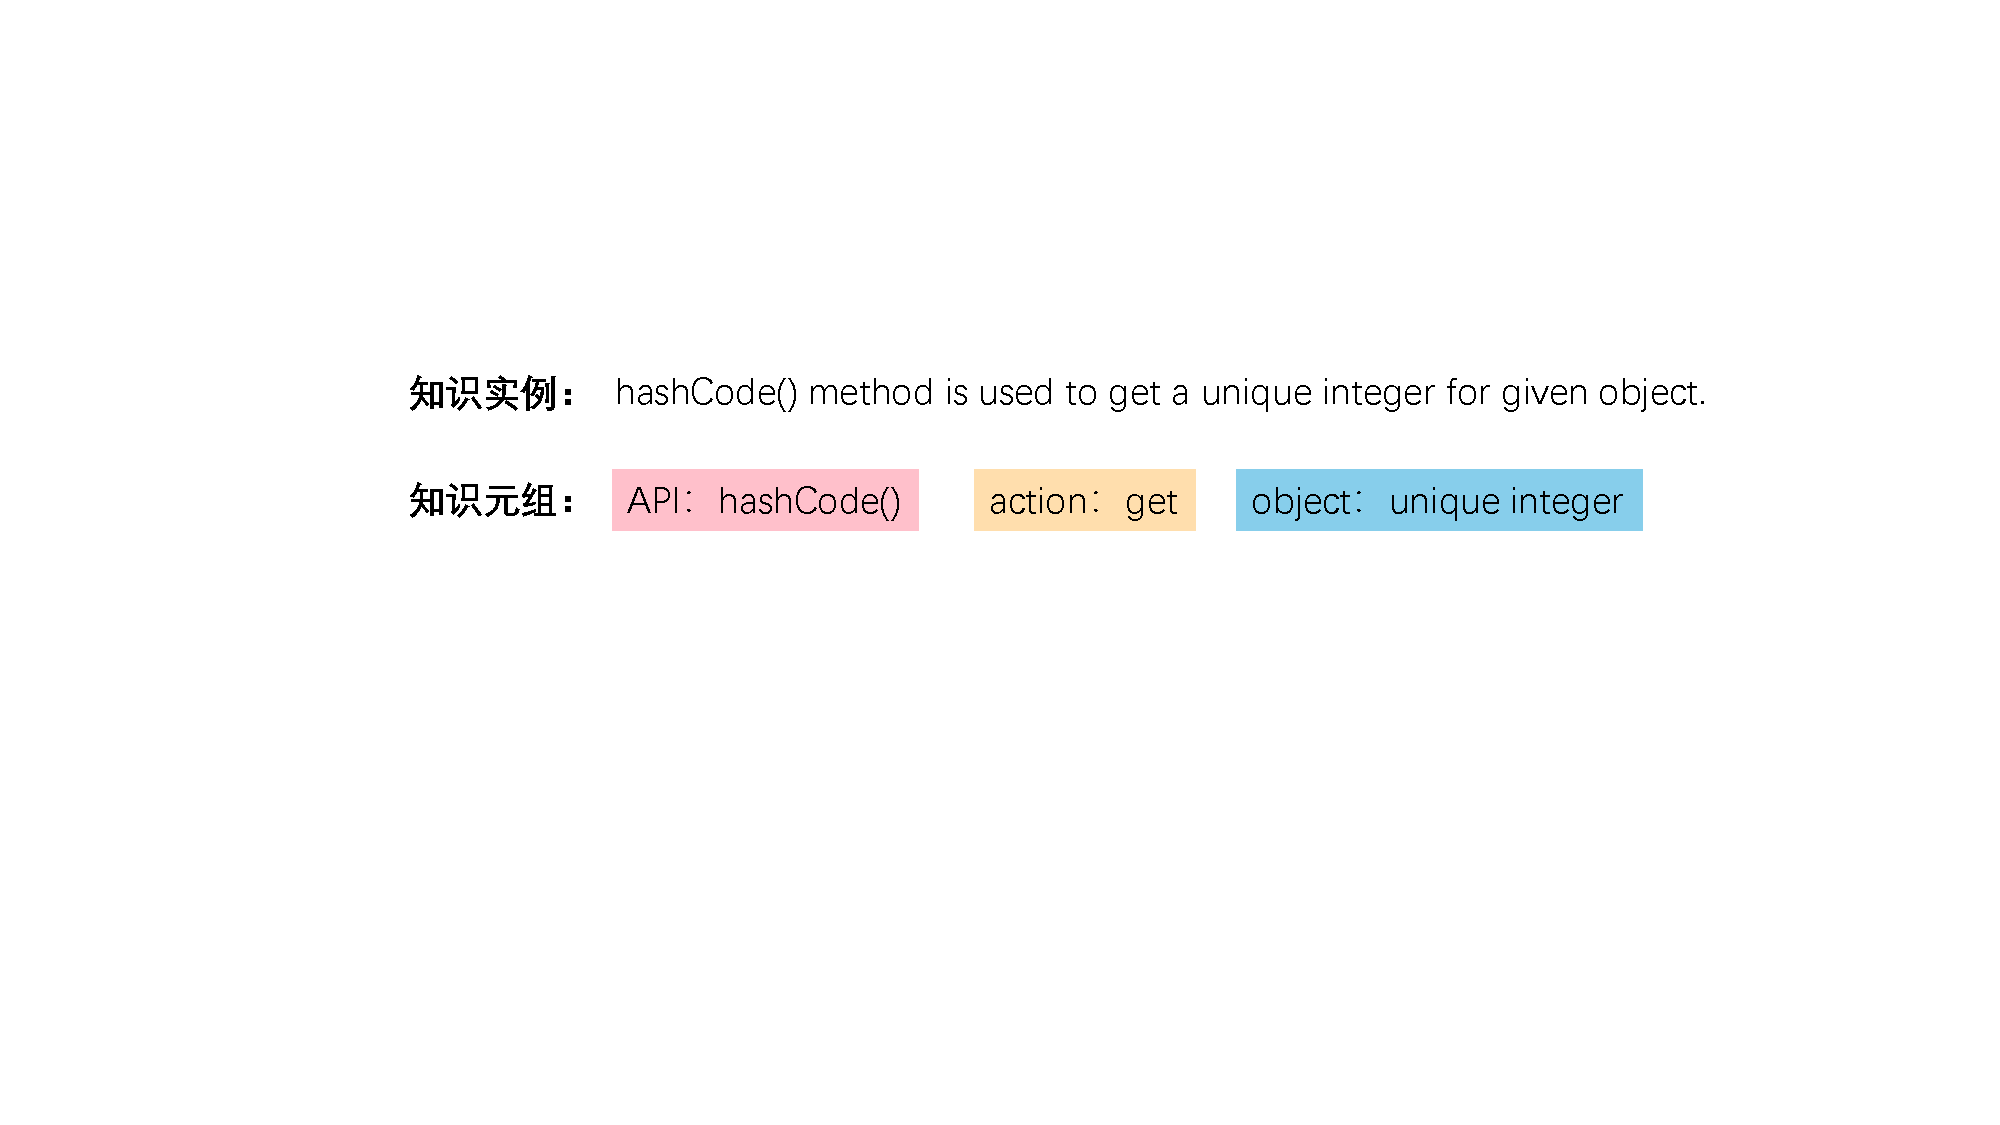
\includegraphics[width=\textwidth]{image/instance.pdf}
    \caption{API描述性知识元组及其实例示例} 
    \label{fig:fig1} 
\end{figure}

\begin{itemize}
    \item 完整性:这个实例是否完整地描述了一个API描述性知识,没有缺失必要的信息。
    \item 有用性:掌握这个API描述性知识是否对软件开发有所帮助,是否能在软件开发的过程中使用到。
    \item 可理解性:这个API描述性知识元组是否能让人快速的理解完整的API描述性知识实例。
\end{itemize}
评分从0分到3分,0分表示非常不同意,1分表示部分不同意,2分表示部分同意,3分表示非常同意。

\subsection{实验结果分析}
图\ref{fig:fig2}为本章节实验的评分结果。在本章节的实验中,综合两位标注者对于API描述性知识的完整性评分,有26\%的评分为3分,59\%的评分为2分,而负面评价的1分和0分分别占12\%和3\%。对于API实例的有用性评分,32\%的评分为3分,53\%的评分为2分,评分为1分的有13\%,剩余2\%的评分是0分。而在可理解性方面,正面评分的3分和2分的比例分别是7\%和58\%,负面评价的1分和0分的比例则为28\%和7\%。两位参与者在完整性、有用性、可理解性三个方面的平均评分分别为2.08、2.16、1.58和2.08、2.14、1.72。	

\begin{figure}[htb]
    \centering
    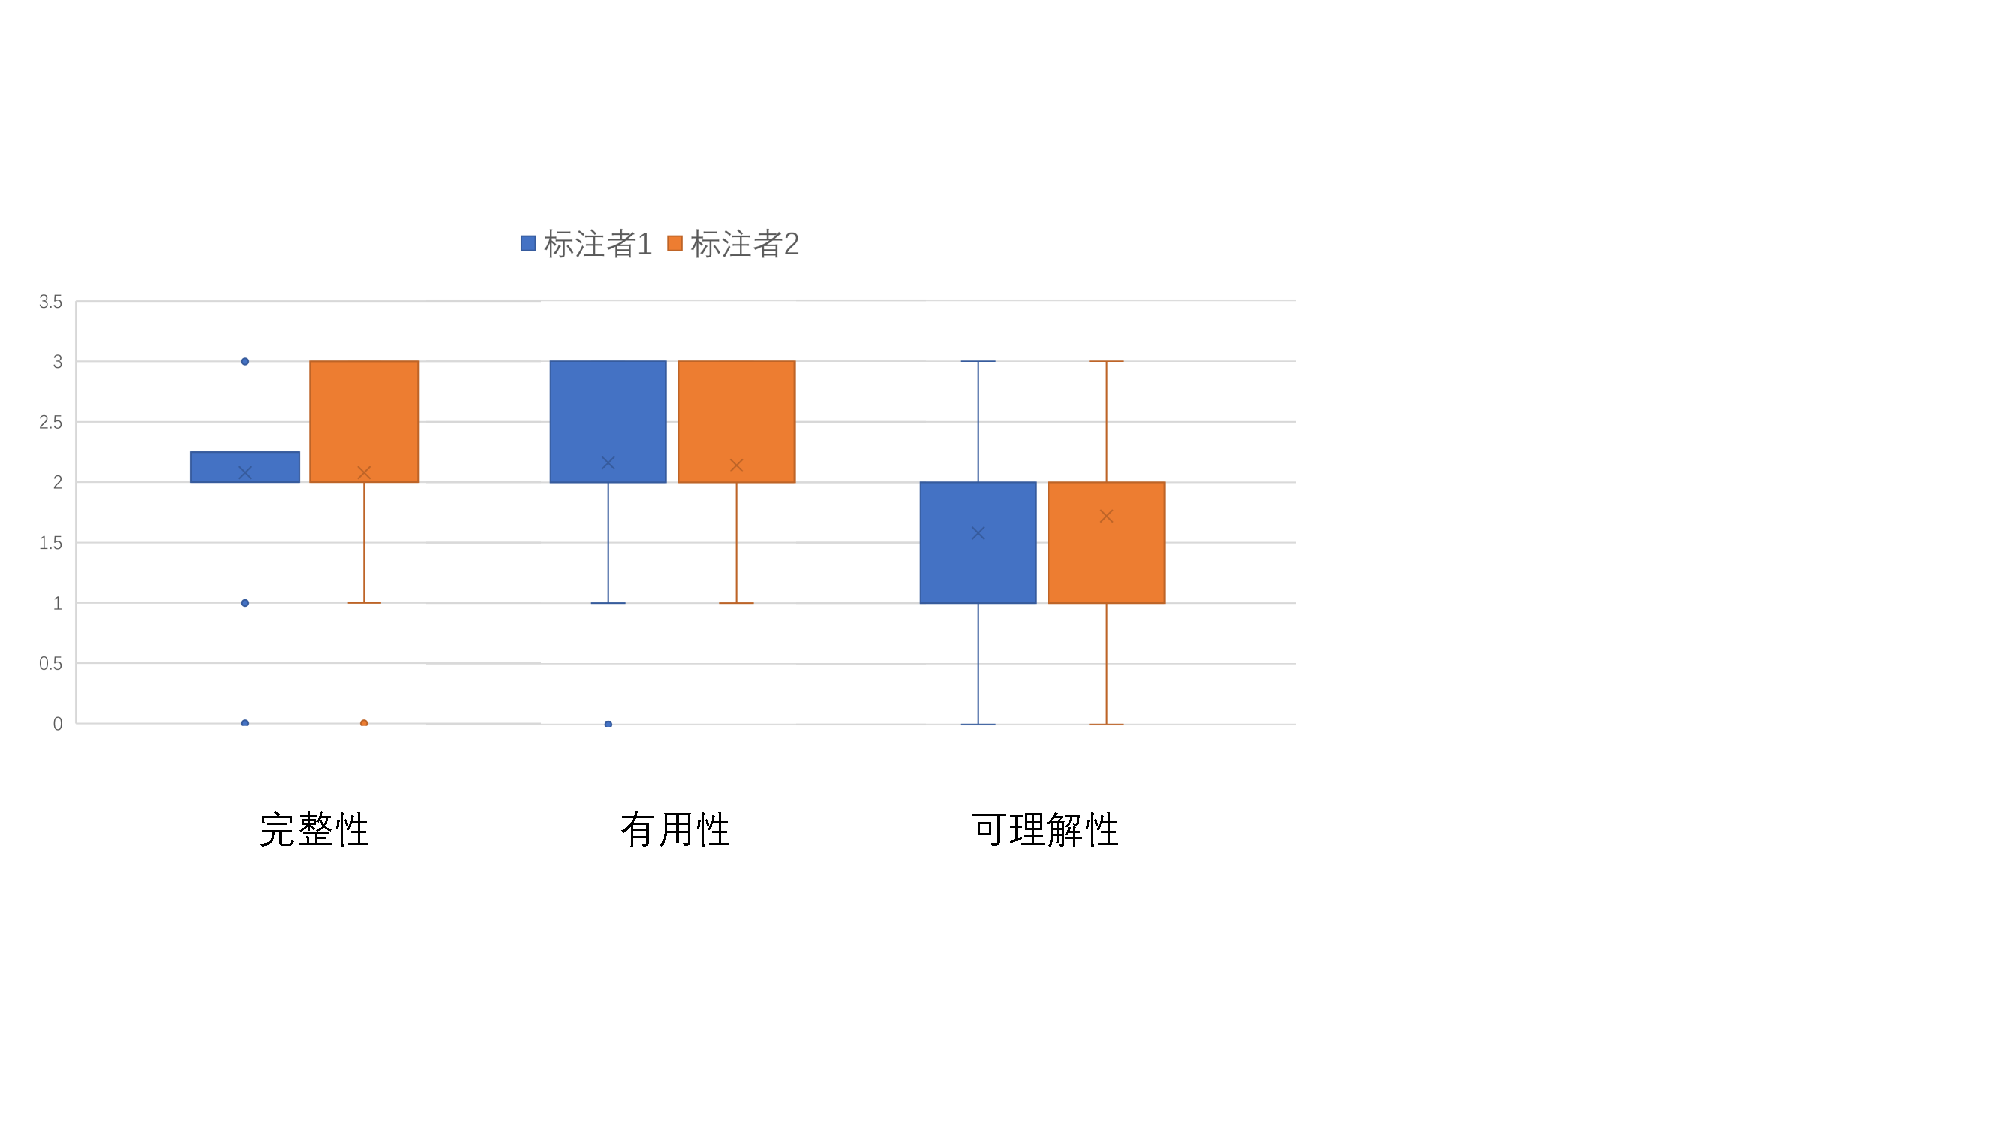
\includegraphics[width=\textwidth]{image/youxiaoxing.pdf}
    \caption{API描述性知识有效性评估实验结果} 
    \label{fig:fig2} 
\end{figure}

为了保证两位参与者的打分情况的显著性差异,本文对两位参与者的评分数据进行了双样本的T检验。在T检验的结果中,如果显著性水平值p<0.05,则可以说明两组数据之间存在显著的差异。而在本章节的实验结果中,计算得到的显著性水平值p为0.047,小于0.05,因此两组数据之间确实是存在显著性差异的。

从以上数据中可以得知,本方法抽取得到的API描述性知识实例在完整性、有用性方面是较为优秀的,平均评分达到了2.08和2.15,说明实验参与者认为本方法抽取出的API描述性知识实例在软件开发的过程中能够有效地帮助到程序员。

对实验数据中完整性和有用性被评为0分的API描述性知识实例进行分析,本文发现它们主要有以下特点:

\begin{enumerate}
    \item 实例中同时包含多个动作元素以及多个目标对象元素。由于本方法中的知识元组匹配环节中,只要一个句子中包含知识元组中的所有元素,就可以匹配得到一个知识实例,所以一个缺失元素的知识元组也有可能匹配上一个知识实例。
    \item 实例中描述的知识内容不完整。由于本文实现的是句子级别的API描述性知识抽取,所以本方法对一个由多个句子组成的API描述性知识的抽取效果较差。当遇到这种多句子API描述性知识时,本系统只能抽取出残缺的知识,这些知识的有用性较差。
\end{enumerate}

针对上述第一个问题,可以考虑在抽取出API描述性知识实例后,基于实例中的词语对匹配的API描述性知识元组进行补全。这样就能有效提高本文抽取出来的API描述性知识的完整性。针对第二个问题,如果未来能实现将细粒度和粗粒度的知识抽取方式相结合的抽取方法,可以克服这一缺点。

而在可理解性方面,本方法抽取出的API描述性知识元组的可理解性较为一般,因为一个完整的API描述性知识句子的语义较为复杂,而本方法抽取出的API描述性知识元素数量有限,且没有上下文信息,这种抽象化的结构表达对于人来说是比较难理解的。但抽象化的结构表达对于帮助机器理解语义有非常大的帮助,且结构化的API描述性知识元组能帮助本系统构建成带有层次关系的知识图谱,便于通过API知识元素和API描述性知识元组之间的关系进行检索。如在本文构建得到的API描述性知识图谱中,只要搜索所有与“thread-safe”这个characteristic之间有has characteristic关系的API描述性知识及其实例,就能实现对thread-safe这个API特性的范围检索,找到所有带有thread-safe特性的API。

\subsection{API描述性知识的有效性评估实验总结}
通过上文中的实验分析,我们可以认为本方法中抽取出来的API描述性知识实例在完整性、有用性方面较为优秀,抽取出来的API描述性知识元组也能够在软件开发的过程中对程序员有所帮助,且API描述性知识元组的结构化表达也为本系统构建知识图谱提供了帮助,方便根据图谱中的关系进行检索。

\section{API描述性知识汇总应用对API文档的互补性评估实验}
在验证完本方法抽取出来的API描述性知识的有效性基础之上,本章节将继续讨论这些知识能否对API文档进行补充。章节4.4介绍了本文实现的API描述性知识汇总应用,本章节设计的实验将邀请开发者使用该应用,并对该应用给出的API描述性知识是否能对API文档完成补充进行评价。

\subsection{实验设计}
首先从本文中构建的API描述性知识图谱中检索出包含API描述性知识实例数量大于10条的API节点,共有309个,在其中随机选择20个作为目标API。然后依旧是邀请两位硕士研究生,请他们使用本文实现的汇总应用查询目标API,并判断系统左侧展示的API描述性知识实例能否作为系统右侧展示的API文档的补充知识。系统的具体展示页面详见图4-1。

本实验的内容同样是对API描述性知识实例进行打分,要求两位实验参与者对系统左侧展示的前五条API描述性知识实例评分,即一共对100条API描述性知识实例进行评估。打分的标准从0到3分,0分表示完全无法作为API文档的补充,1分表示这条API描述性知识实例已经包含在API文档里了,2分表示API描述性知识实例中的部分表述可以作为文档的补充,3分表示这个知识实例可以完整地补充到API文档中。

\subsection{实验结果分析}
实验结果统计如图\ref{fig:fig3}所示。综合两位标注者的评分结果来看,有19.5\%的评分是3分,49\%的评分是2分,标注为1分的评分有22\%,最后还有9.5\%的API描述性知识实例被评为0分。所有API描述性知识实例的平均评分是1.785。单独对每一个随机选取的API来看,每个API相关的5条API描述性知识实例中,平均有0.98条知识实例被评为3分,2.45条知识实例被评为2分,作为负面评价的1分和0分分别有1.1条和0.48条。从实验结果中可以得知,本方法抽取出来的API描述性知识对于API文档具有良好的补充作用,随机采样得到的100条API描述性知识实例的平均评分为1.785,表示这些知识实例大多是对于补充API文档具有正面作用的。

\begin{figure}[htb]
    \centering
    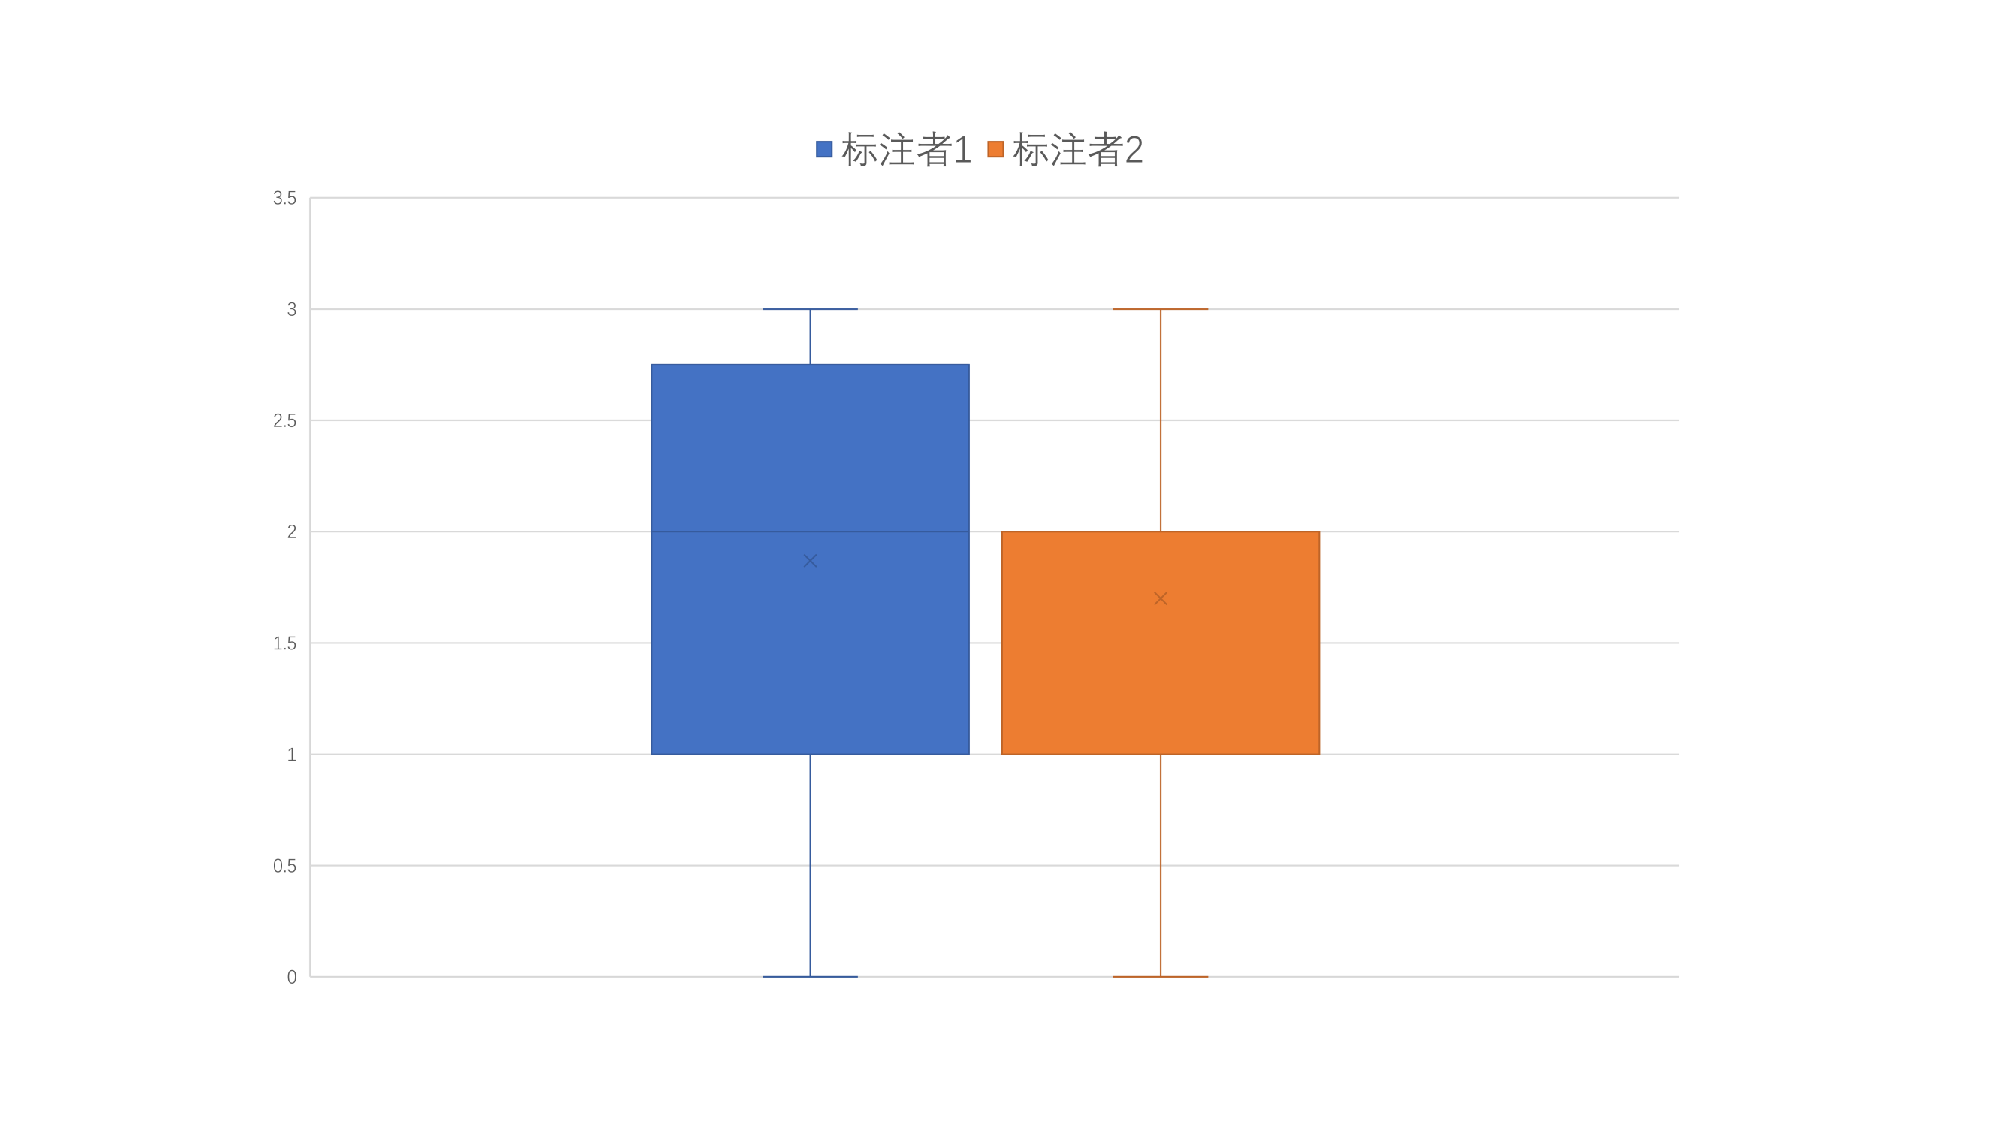
\includegraphics[width=\textwidth]{image/5-2.pdf}
    \caption{API描述性知识汇总应用与API文档互补性评估实验结果} 
    \label{fig:fig3} 
\end{figure}

由于本方法在进行API描述性知识的抽取之前,对语料库进行了多项过滤工作,保证了语料库中API描述性知识句子的覆盖率,所以本方法抽取得到的API描述性知识的有效性是具有保障的,前文章节5.3所设计的实验也证明了这一点。但在本系统抽取得到的知识中,部分API描述性知识来自于原作者在帖子中引用API文档中已有的知识,或者用自己的语言重新描述一个API文档中已存在的知识点,这种API描述性知识在本方法的挖掘结果中占了22\%。

除此之外,实验结果中还存在49\%的API描述性知识实例被评为2分。这些知识实例既包括了API文档中已有的知识点,也存在部分不在API文档之中的知识。开发者们在Stack Overflow上讨论一个API时,可能会加上自己对这个API的理解,或者对已有的API知识进行深入的拓展讨论,比如分析一个API的特性是如何在底层实现的。我们认为这种API描述性知识实例对于API文档的补充是具有正面价值的。

对于这些与API文档包含有重复知识的API描述性知识实例,如果能基于API文档本身对本系统抽取出来的知识实例进行过滤,那么剩余的知识实例的有效性将会大大提升。可以考虑使用基于句子相似度的过滤方式对本文抽取出来的知识实例进行去重,如对API文档进行分句,然后计算API描述性知识实例与文档中的每一个句子的句子相似度。如果该实例与API文档里的其中一个句子相似度很高,就将这个实例过滤掉。这样经过过滤后,本系统实现的应用对于API文档的互补性应该会大大提升。

最后,由于API文档对一个API的表述非常简洁,只取重点,大多数API文档仅仅是对API的功能、输入以及输出进行介绍。而在Stack Overflow上,开发者们对一个API的讨论可能会深入到源码层面,或者对一个API在实际编程过程中的表现、特性等进行讨论,所以本文方法能够在这种讨论中抽取出不存在于API文档中的知识。

\subsection{API描述性知识汇总应用的有效性评估实验总结}
本章节设计的有效性评估实验证明了本方法抽取出来的API描述性知识实例大多对API官方文档的补充具有一定的价值。其中,部分API描述性知识实例已经被API文档覆盖了,如果能够提出一种过滤机制对抽取出来的API描述性知识再进行一次筛选,过滤掉那些已经在文档中存在的知识,那么本方法抽取出来的API描述性知识的价值将会大大提高。

\section{方法有效性威胁}
本方法的有效性威胁主要分为两个部分,分别是存在于本文方法之中的内部有效性威胁和除此之外的外部有效性威胁。

\subsection{内部有效性威胁}
在本文的知识抽取流程中,面临的内部有效性威胁来自于本方法所使用的一些外部工具,包括fastText文本分类器和自然语言处理工具spaCy。在生成语料库的时候,本方法使用了fastText文本分类技术,用于从包含API提及的句子中识别出API描述性知识句子。尽管fastText分类器的文本分类效果很好,但仍不能达到100\%的分类准确率。当一个非API描述性知识句子被分类为正样本时,这个句子可能在抽取过程中并不会被匹配上,也可能会从这个句子中抽取出错误的API描述性知识元组。而在本文的抽取流程中,一个错误的抽取结果会像一个雪球一样在多次迭代后越滚越大,形成更多错误的知识和语言模式,这样会对本方法抽取得到的结果产生不良影响。为了保证本方法的有效性,本文在抽取流程中设置了严格的过滤条件,用于筛选掉错误、低质量的API描述性知识元组。本文的实验评估证明过滤机制是有效的,但分类错误带来的影响依然部分存在于抽取结果中。

而自然语言处理工具spaCy的性能也对本方法的有效性有着举足轻重的影响。spaCy在自然语言解析的过程中出现的分词、分句错误都会对本方法带来负面影响。虽然spaCy的性能在自然语言处理领域是非常优秀的,且它在被应用于软件工程相关文本的时候相比其他工具有着更好的表现,但目前也并没有哪个自然语言处理工具能够在处理大规模语料时保证100\%的准确率。本文方法中,Stack Overflow帖子的分句依赖于spaCy的句子解析模块,API描述性知识实例的语言模式抽取也依赖于spaCy的词语解析模块。虽然本方法使用了贴近于Stack Overflow网站文本的定制化分句、分词规则,且在语言模式匹配时将单词数量阈值设置为4个以提高分词容错率,但依然会因为文本自身的一些问题导致分词分句的错误(如前文章节5.1.2所述),以及语言模式抽取的错误。

\subsection{外部有效性威胁}
本文面对的外部有效性威胁主要来自于实验评估环节,以及方法的泛用性相关问题。
在实验评估环节中,本文设计的部分实验具有较强的主观性,且实验的规模较小。如章节5.3以及章节5.4所设计的实验,均采用了人工评分的方式来对本文抽取的结果进行评估,而且抽样的实例数量只有100条。为了减轻实验参与者的主观性对本方法造成的影响,本文邀请的标注者首先要求具有3年以上的Java语言开发经验,这确保了他们对于Java语言的API知识是足够熟悉的。其次,本文在实验部分均至少邀请了两位参与者,并且在得到实验结果后设计了T检验对结果进行检查,确保两人的评分结果是存在显著性差异的。但实验规模较小带来的有效性威胁仍然是客观存在的。

此外,由于本方法的语料库生成模块只选用了带有Java标签的Stack Overflow帖子,且实验评估也是针对Java语言所设计的,并没有对其他的编程语言帖子进行抽取和实验,所以还不能确保本方法在其他编程语言上具有泛用性。

\section{本章小结}
本章节中,首先提出了3个问题,分别从系统流程的有效性以及系统产出的有效性两个方面入手进行讨论,并设计了一系列实验,分别验证了本文流程中语料库生成模块与抽取主体模块的有效性以及本文方法抽取出的API描述性知识实例的有效性。对于本文实现的API描述性知识汇总应用,本文还设计了与API文档的补充实验,证明本文方法抽取得到的部分API描述性知识实例能够作为API文档的补充,是具有一定价值的。在本章的最后,还对本文面临的内部有效性威胁和外部有效性威胁进行了讨论。
